% !TeX root = ../libro.tex
% !TeX encoding = utf8



\setchapterpreamble[c][0.75\linewidth]{%
	\sffamily
  
    En este capítulo se mostraran los resultados obtenidos de dos de los cuatro mejores modelos de la competición, los resultados obtenido de los modelos propuestos por la literatura y los resultados de los modelos propios. Además, para la elección de los hiperparámetros óptimos en las propuestas propias de modelo, se ha realizado un proceso experimental el cual también se expondrá. Tras ello, se procederá a realizar un análisis detenido en detalle sobre los resultados obtenidos que culminará con una comparación entre todos los modelos.
  

	\par\bigskip
}

\chapter{Resultados y Análisis}\label{ch:analisis}


%%%%%%%%%%%%%%%%%%%%%%%%%%%%%%%%%%%%%%%%%%%%%%%%%%%%%%%%%%%%%%%%%%%%%%%%%%%%%%%%%%%%%%%%
%%%%%%%%%%%%%%%%%%%%%%%%%%%%%%%%%%%%%%%%%%%%%%%%%%%%%%%%%%%%%%%%%%%%%%%%%%%%%%%%%%%%%%%%
%%%%%%%%%%%%%%%%%%%%%%%%%%%%%%%%%%%%%%%%%%%%%%%%%%%%%%%%%%%%%%%%%%%%%%%%%%%%%%%%%%%%%%


\section{Resultados}

    En esta sección presentamos los resultados de los modelos anteriormente comentados a excepción del marco de interpretación abductivo y el modelo ENCASE, los cuales no han podido ser reproducidos.
    
    \subsection{Modelos ganadores de la competición}
    

        \begin{table}[H]
        \caption{Resultados de dos de los cuatro modelos ganadores. Clasificador basado en Randon Forest y Clasificador Binario en Cascada}
        \begin{center}
        \begin{tabular}{|c|r|r|}
        \hline
        & \multicolumn{1}{l|}{\textbf{Clasif. Random Forest}} & \multicolumn{1}{l|}{\textbf{Clasif. B. Cascd.}} \\ \hline
        \textbf{Fn} & 0,916 & 0,892 \\ \hline
        \textbf{Fa} & 0,827 & 0,768 \\ \hline
        \textbf{Fo} & 0,786 & 0,722 \\ \hline
        \textbf{Fr} & 0,617 & 0,584 \\ \hline
        \textbf{F1} & 0,787 & 0,741 \\ \hline
        \end{tabular}
        \end{center}
        \label{table:resultados_modelosganadores}
        \end{table}

        \begin{table}[H]
        \caption{Matriz de Confusión del clasificador basado en Random Forest}
        \begin{center}
        \begin{tabular}{|c|r|r|r|r|}
        \hline
        \multicolumn{1}{|l|}{} & \multicolumn{1}{l|}{\textbf{Normal}} & \multicolumn{1}{l|}{\textbf{FA}} & \multicolumn{1}{l|}{\textbf{Otro}} & \multicolumn{1}{l|}{\textbf{Ruido}} \\ \hline
        \textbf{Normal} & 953 & 2 & 57 & 3 \\ \hline
        \textbf{FA} & 5 & 116 & 29 & 2 \\ \hline
        \textbf{Otro} & 92 & 10 & 375 & 6 \\ \hline
        \textbf{Ruido} & 15 & 1 & 10 & 29 \\ \hline
        \end{tabular}
        \end{center}
        \label{table:RF_CM}
        \end{table}


    

        \begin{table}[H]
        \caption{Matriz de confusión del clasificador binario en cascada}
        \begin{center}
        \begin{tabular}{|c|r|r|r|r|}
        \hline
        \multicolumn{1}{|l|}{} & \multicolumn{1}{l|}{\textbf{Normal}} & \multicolumn{1}{l|}{\textbf{FA}} & \multicolumn{1}{l|}{\textbf{Otro}} & \multicolumn{1}{l|}{\textbf{Ruido}} \\ \hline
        \textbf{Normal} & 962 & 7 & 53 & 6 \\ \hline
        \textbf{FA} & 6 & 114 & 28 & 4 \\ \hline
        \textbf{Otro} & 118 & 21 & 333 & 10 \\ \hline
        \textbf{Ruido} & 15 & 4 & 7 & 31 \\ \hline
        \end{tabular}
        \end{center}
        \label{table:CBC_CM}
        \end{table}


    
    
    
    \subsection{Modelos propuestos por la literatura}
    
    
          
        \begin{table}[H]
        \caption{Matriz de Confusión GaoJunLi}
        \begin{center}
        \begin{tabular}{|l|r|r|r|r|}
        \hline
         & \multicolumn{1}{l|}{\textbf{Normal}} & \multicolumn{1}{l|}{\textbf{FA}} & \multicolumn{1}{l|}{\textbf{Otro}} & \multicolumn{1}{l|}{\textbf{Ruido}} \\ \hline
        \textbf{Normal} & 1011 & 0 & 0 & 0 \\ \hline
        \textbf{FA} & 147 & 0 & 0 & 0 \\ \hline
        \textbf{Otro} & 491 & 0 & 0 & 0 \\ \hline
        \textbf{Ruido} & 57 & 0 & 0 & 0 \\ \hline
        \end{tabular}
        \end{center}
        \label{table:GaoJunLin_CM}
        \end{table}
        
        
        \begin{table}[H]
        \caption{Matriz de Confusión del modelo ChenChen}
        \begin{center}
        \begin{tabular}{|l|r|r|r|r|}
        \hline
         & \multicolumn{1}{l|}{\textbf{Normal}} & \multicolumn{1}{l|}{\textbf{FA}} & \multicolumn{1}{l|}{\textbf{Otro}} & \multicolumn{1}{l|}{\textbf{Ruido}} \\ \hline
        \textbf{Normal} & 873 & 2 & 92 & 0 \\ \hline
        \textbf{FA} & 122 & 1 & 11 & 0 \\ \hline
        \textbf{Otro} & 431 & 2 & 43 & 0 \\ \hline
        \textbf{Ruido} & 38 & 0 & 1 & 0 \\ \hline
        \end{tabular}
        \end{center}
        \label{table:ChenChen_CM}
        \end{table}
        
        \begin{table}[H]
        \caption{Matriz de Confusión del modelo OhShuLi}
        \begin{center}
        \begin{tabular}{|l|r|r|r|r|}
        \hline
         & \multicolumn{1}{l|}{\textbf{Normal}} & \multicolumn{1}{l|}{\textbf{FA}} & \multicolumn{1}{l|}{\textbf{Other}} & \multicolumn{1}{l|}{\textbf{Ruido}} \\ \hline
        \textbf{Normal} & 980 & 0 & 29 & 0 \\ \hline
        {\textbf{FA}} & 141 & 0 & 6 & 0 \\ \hline
        \textbf{Other} & 470 & 0 & 20 & 0 \\ \hline
        \textbf{Ruido} & 52 & 0 & 5 & 0 \\ \hline
        \end{tabular}
        \end{center}
        \label{cm_ohsuli}
        \end{table}

        
        \begin{table}[H]
        \caption{Resultados de los modelos OhShuLi, ChenChen y GaoJunLi}
        \begin{center}
        \begin{tabular}{|l|r|r|r|}
        \hline
         & \multicolumn{1}{l|}{\textbf{GaoJunLi}} & \multicolumn{1}{l|}{\textbf{ChenChen}} & \multicolumn{1}{l|}{\textbf{OhShuLi}} \\ \hline
        \textbf{Test loss} & 0,986 & 1,302 & 0,833 \\ \hline
        \textbf{Test accuracy} & 0,591 & 0,631 & 0,652 \\ \hline
        \textbf{Test sco} & 0,201 & 0,279 & 0,341 \\ \hline
        \textbf{Fn} & 0,743 & 0,776 & 0,793 \\ \hline
        \textbf{Fa} & 0 & 0,149 & 0,193 \\ \hline
        \textbf{Fo} & 0,034 & 0,192 & 0,31 \\ \hline
        \textbf{Fr} & 0,068 & 0,088 & 0,249 \\ \hline
        \textbf{F1} & 0,211 & 0,301 & 0,386 \\ \hline
        \end{tabular}
        \end{center}
        \label{table:results_litera}
        \end{table}


        \begin{figure}[H]
            \centering
            \includegraphics[width=\textwidth,height=\textheight,keepaspectratio]{img/ChenChen_epoch_sco.png}
            \caption{Modelo ChenChen - El eje X representa el avance de las épocas y el eje Y la métrica $F_1$. La curva naranja representa el entrenamiento y la azul la validación.}
            \label{fig:chenchen_tensorboard}
        \end{figure}
        
        \begin{figure}[H]
            \centering
            \includegraphics[width=\textwidth,height=\textheight,keepaspectratio]{img/ohshuli_epoch_sco.png}
            \caption{Modelo OhShuLi - El eje X representa el avance de las épocas y el eje Y la métrica $F_1$.La curva naranja representa el entrenamiento y la azul la validación.}
            \label{fig:ohshuli_tensorboard}
        \end{figure}
        
        \begin{figure}[H]
            \centering
            \includegraphics[width=\textwidth,height=\textheight,keepaspectratio]{img/GaoJunLi_epochsco.png}
            \caption{Modelo GaoJunLi - El eje X representa el avance de las épocas y el eje Y la métrica $F_1$.La curva naranja representa el entrenamiento y la azul la validación.}
            \label{fig:gaojunli_tensorboard}
        \end{figure}
    
    
    
    \subsection{Modelos propios}
    
    
    \begin{table}[H]
    \caption{Resultados de la fase de experimentación del modelo LSTM. Los resultados están ordenados de manera decreciente según el valor de la métrica $F_1$.}
    \begin{center}
    \begin{tabular}{|r|r|r|l|r|r|r|r|r|}
    \hline
    \multicolumn{1}{|l|}{} & \multicolumn{1}{l|}{\textbf{lstm\_units}} & \multicolumn{1}{l|}{\textbf{dense\_units}} & \textbf{padding} & \multicolumn{1}{l|}{\textbf{Fn}} & \multicolumn{1}{l|}{\textbf{Fa}} & \multicolumn{1}{l|}{\textbf{Fo}} & \multicolumn{1}{l|}{\textbf{Fr}} & \multicolumn{1}{l|}{\textbf{F1}} \\ \hline
    1 & 16 & 32 & same & 0,8485 & 0,3117 & 0,5246 & 0,3611 & 0,5115 \\ \hline
    2 & 16 & 32 & valid & 0,8394 & 0,3457 & 0,5273 & 0,2632 & 0,4939 \\ \hline
    3 & 16 & 8 & valid & 0,8409 & 0,2221 & 0,5166 & 0,1543 & 0,4335 \\ \hline
    4 & 8 & 8 & same & 0,8042 & 0,5443 & 0,3057 & 0,0000 & 0,4136 \\ \hline
    5 & 16 & 8 & same & 0,8457 & 0,1243 & 0,5321 & 0,1307 & 0,4082 \\ \hline
    6 & 8 & 32 & same & 0,7914 & 0,3447 & 0,3572 & 0,1055 & 0,3997 \\ \hline
    7 & 8 & 32 & valid & 0,7945 & 0,2970 & 0,2949 & 0,1675 & 0,3885 \\ \hline
    8 & 4 & 8 & valid & 0,7864 & 0,3630 & 0,1944 & 0,0000 & 0,3360 \\ \hline
    9 & 8 & 8 & valid & 0,7889 & 0,2269 & 0,2939 & 0,0000 & 0,3274 \\ \hline
    10 & 4 & 8 & same & 0,7885 & 0,2576 & 0,2581 & 0,0000 & 0,3261 \\ \hline
    11 & 4 & 32 & valid & 0,7593 & 0,0425 & 0,1605 & 0,0000 & 0,2406 \\ \hline
    12 & 4 & 32 & same & 0,7412 & 0,0000 & 0,0859 & 0,0000 & 0,2068 \\ \hline
    \end{tabular}
    \end{center}
    \label{table:model2_result}
    \end{table}
    
    \begin{table}[htbp]
        \caption{Resultados de la fase de experimentación del primer modelo GRU. Los resultados están ordenados de manera decreciente según el valor de la métrica $F_1$.}
        \begin{center}
        \begin{tabular}{|r|l|r|r|r|r|r|r|r|}
        \hline
        \multicolumn{1}{|l|}{} & \textbf{drop} & \multicolumn{1}{l|}{\textbf{gru\_units}} & \multicolumn{1}{l|}{\textbf{dense\_units}} & \multicolumn{1}{l|}{\textbf{Fn}} & \multicolumn{1}{l|}{\textbf{Fa}} & \multicolumn{1}{l|}{\textbf{Fo}} & \multicolumn{1}{l|}{\textbf{Fr}} & \multicolumn{1}{l|}{\textbf{F1}} \\ \hline
        1 & 0.4 & 25 & 32 & 0,8715 & 0,6682 & 0,5921 & 0,4415 & 0,6433 \\ \hline
        2 & 0.4 & 25 & 64 & 0,8699 & 0,6681 & 0,5871 & 0,4308 & 0,6390 \\ \hline
        3 & 0.4 & 16 & 32 & 0,8642 & 0,5345 & 0,5428 & 0,4751 & 0,6042 \\ \hline
        4 & 0.4 & 16 & 32 & 0,8591 & 0,5949 & 0,5284 & 0,3728 & 0,5888 \\ \hline
        5 & 0.4 & 16 & 64 & 0,8566 & 0,5208 & 0,5411 & 0,3722 & 0,5727 \\ \hline
        6 & 0.4 & 4 & 8 & 0,7586 & 0,2969 & 0,2170 & 0,0795 & 0,3380 \\ \hline
        7 & 0.4 & 16 & 8 & 0,8333 & 0,0000 & 0,4466 & 0,0069 & 0,3217 \\ \hline
        8 & 0.4 & 8 & 32 & 0,8027 & 0,1059 & 0,3110 & 0,0389 & 0,3146 \\ \hline
        9 & 0.4 & 8 & 8 & 0,7670 & 0,0000 & 0,1165 & 0,0000 & 0,2209 \\ \hline
        10 & 0.4 & 4 & 32 & 0,7438 & 0,0000 & 0,0000 & 0,0000 & 0,1860 \\ \hline
        \end{tabular}
        \end{center}
        \label{table:model3_result}
        \end{table}
    

        \begin{table}[H]
        \caption{Resultados de la fase de experimentación del modelo CNN. Los resultados están ordenados de manera decreciente según el valor de la métrica $F_1$.}
        \begin{center}
        \resizebox{\columnwidth}{!}{%
        \begin{tabular}{|r|l|r|r|l|r|r|r|r|r|}
        \hline
        \multicolumn{1}{|l|}{\textbf{Nº}} & \textbf{drop} & \multicolumn{1}{l|}{\textbf{filters}} & \multicolumn{1}{l|}{\textbf{kernel}} & \textbf{padding} & \multicolumn{1}{l|}{\textbf{Fn}} & \multicolumn{1}{l|}{\textbf{Fa}} & \multicolumn{1}{l|}{\textbf{Fo}} & \multicolumn{1}{l|}{\textbf{Fr}} & \multicolumn{1}{l|}{\textbf{F1}} \\ \hline
        1 & 0.4 & 256 & 9 & same & 0,8785 & 0,7360 & 0,6340 & 0,5194 & 0,6920 \\ \hline
        2 & 0.4 & 256 & 7 & same & 0,8809 & 0,7393 & 0,6457 & 0,4893 & 0,6888 \\ \hline
        3 & 0.4 & 128 & 3 & same & 0,8802 & 0,7384 & 0,6378 & 0,4834 & 0,6850 \\ \hline
        4 & 0.4 & 128 & 5 & same & 0,8830 & 0,7144 & 0,6359 & 0,5062 & 0,6849 \\ \hline
        5 & 0.2 & 128 & 3 & same & 0,8800 & 0,7309 & 0,6469 & 0,4676 & 0,6814 \\ \hline
        6 & 0.2 & 64 & 5 & same & 0,8790 & 0,7221 & 0,6233 & 0,4831 & 0,6769 \\ \hline
        7 & 0.4 & 128 & 3 & same & 0,8808 & 0,7137 & 0,6325 & 0,4757 & 0,6757 \\ \hline
        8 & 0.4 & 128 & 7 & same & 0,8819 & 0,7345 & 0,6481 & 0,4294 & 0,6735 \\ \hline
        9 & 0.4 & 256 & 3 & same & 0,8808 & 0,7137 & 0,6508 & 0,4443 & 0,6724 \\ \hline
        10 & 0.4 & 512 & 3 & same & 0,8768 & 0,7237 & 0,6310 & 0,4561 & 0,6719 \\ \hline
        11 & 0.2 & 128 & 5 & valid & 0,8749 & 0,7080 & 0,6217 & 0,4740 & 0,6696 \\ \hline
        12 & 0.4 & 128 & 5 & valid & 0,8743 & 0,7248 & 0,6062 & 0,4519 & 0,6643 \\ \hline
        13 & 0.2 & 128 & 3 & valid & 0,8741 & 0,7019 & 0,6129 & 0,4652 & 0,6635 \\ \hline
        14 & 0.4 & 128 & 3 & valid & 0,8725 & 0,6875 & 0,6102 & 0,4479 & 0,6545 \\ \hline
        15 & 0.2 & 64 & 3 & same & 0,8711 & 0,6887 & 0,5844 & 0,4525 & 0,6492 \\ \hline
        16 & 0.2 & 64 & 3 & valid & 0,8683 & 0,6675 & 0,5830 & 0,4663 & 0,6463 \\ \hline
        17 & 0.2 & 64 & 5 & valid & 0,8667 & 0,6701 & 0,5730 & 0,4306 & 0,6351 \\ \hline
        18 & 0.4 & 64 & 5 & valid & 0,8678 & 0,6663 & 0,5655 & 0,4223 & 0,6305 \\ \hline
        19 & 0.4 & 64 & 3 & valid & 0,8655 & 0,6680 & 0,5518 & 0,4187 & 0,6260 \\ \hline
        20 & 0.2 & 32 & 5 & same & 0,8642 & 0,6292 & 0,5408 & 0,4167 & 0,6127 \\ \hline
        21 & 0.4 & 128 & 9 & same & 0,8530 & 0,5855 & 0,5167 & 0,4097 & 0,5912 \\ \hline
        22 & 0.4 & 128 & 5 & same & 0,8537 & 0,5833 & 0,5160 & 0,4072 & 0,5900 \\ \hline
        23 & 0.2 & 128 & 5 & same & 0,8532 & 0,5829 & 0,5202 & 0,3860 & 0,5856 \\ \hline
        24 & 0.4 & 256 & 5 & same & 0,8525 & 0,5921 & 0,5193 & 0,3671 & 0,5827 \\ \hline
        25 & 0.4 & 64 & 5 & same & 0,8492 & 0,5731 & 0,4794 & 0,3866 & 0,5721 \\ \hline
        26 & 0.4 & 64 & 3 & same & 0,8453 & 0,4730 & 0,4599 & 0,4012 & 0,5449 \\ \hline
        27 & 0.4 & 32 & 3 & same & 0,8552 & 0,3575 & 0,4957 & 0,3792 & 0,5219 \\ \hline
        28 & 0.2 & 32 & 3 & same & 0,8492 & 0,3099 & 0,5126 & 0,3674 & 0,5098 \\ \hline
        29 & 0.2 & 32 & 3 & valid & 0,8516 & 0,2824 & 0,5466 & 0,3524 & 0,5082 \\ \hline
        30 & 0.2 & 32 & 5 & valid & 0,8533 & 0,2384 & 0,5265 & 0,3087 & 0,4817 \\ \hline
        31 & 0.4 & 512 & 9 & same & 0,8244 & 0,4191 & 0,3801 & 0,2798 & 0,4759 \\ \hline
        32 & 0.4 & 32 & 5 & valid & 0,8512 & 0,0936 & 0,5242 & 0,3929 & 0,4655 \\ \hline
        33 & 0.4 & 32 & 5 & same & 0,8500 & 0,1079 & 0,5182 & 0,3492 & 0,4563 \\ \hline
        34 & 0.4 & 32 & 3 & valid & 0,8469 & 0,0216 & 0,5272 & 0,3184 & 0,4285 \\ \hline
        35 & 0.4 & 512 & 5 & same & 0,7719 & 0,1527 & 0,1282 & 0,0917 & 0,2861 \\ \hline
        36 & 0.4 & 512 & 7 & same & 0,7709 & 0,1478 & 0,1316 & 0,0898 & 0,2850 \\ \hline
        \end{tabular}
        }
        \end{center}
        \label{table:model1_result}
        \end{table}


        
        
        \begin{table}[htbp]
        \caption{Matriz de confusión del modelo GRU}
        \begin{center}
        \begin{tabular}{|l|r|r|r|r|}
        \hline
        \textbf{} & \multicolumn{1}{l|}{\textbf{Normal}} & \multicolumn{1}{l|}{\textbf{FA}} & \multicolumn{1}{l|}{\textbf{Otras}} & \multicolumn{1}{l|}{\textbf{Ruido}} \\ \hline
        \textbf{Normal} & 934 & 6 & 69 & 0 \\ \hline
        \textbf{FA} & 114 & 6 & 27 & 0 \\ \hline
        \textbf{Otras} & 375 & 9 & 106 & 0 \\ \hline
        \textbf{Ruido} & 50 & 1 & 6 & 0 \\ \hline
        \end{tabular}
        \end{center}
        \label{table:CM gru}
        \end{table}

        
      \begin{table}[htbp]
        \caption{Matriz de confusión del modelo LSTM}
        \begin{center}
        \begin{tabular}{|l|r|r|r|r|}
        \hline
        \textbf{} & \multicolumn{1}{l|}{\textbf{Normal}} & \multicolumn{1}{l|}{\textbf{FA}} & \multicolumn{1}{l|}{\textbf{Otras}} & \multicolumn{1}{l|}{\textbf{Ruido}} \\ \hline
        \textbf{Normal} & 927 & 0 & 82 & 0 \\ \hline
        \textbf{FA} & 127 & 0 & 20 & 0 \\ \hline
        \textbf{Otras} & 422 & 0 & 68 & 0 \\ \hline
        \textbf{Ruido} & 51 & 0 & 6 & 0 \\ \hline
        \end{tabular}
        \end{center}
        \label{table:CM lstm}
        \end{table}
  
        \begin{table}[htbp]
        \caption{Matriz de confusión del modelo CNN}
        \begin{center}
        \begin{tabular}{|l|r|r|r|r|}
        \hline
         & \multicolumn{1}{l|}{\textbf{Normal}} & \multicolumn{1}{l|}{\textbf{FA}} & \multicolumn{1}{l|}{\textbf{Otras}} & \multicolumn{1}{l|}{\textbf{Ruido}} \\ \hline
        \textbf{Normal} & 941 & 6 & 62 & 0 \\ \hline
        \textbf{FA} & 117 & 10 & 20 & 0 \\ \hline
        \textbf{Otras} & 371 & 9 & 110 & 0 \\ \hline
        \textbf{Ruido} & 49 & 2 & 6 & 0 \\ \hline
        \end{tabular}
        \end{center}
        \label{table:CM cnn}
        \end{table}


        \begin{figure}[H]
            \centering
            \includegraphics[width=\textwidth,height=\textheight,keepaspectratio]{img/curva modelo 1_best.png}
            \caption{Curva aprendizaje modelo CNN - El eje X representa el avance de las épocas y el eje Y la métrica $F_1$.La curva naranja representa el entrenamiento y la azul la validación.}
            \label{fig:curva_model1}
        \end{figure}
        
        
        
        \begin{figure}[H]
            \centering
            \includegraphics[width=\textwidth,height=\textheight,keepaspectratio]{img/curva modelo2_best.png}
            \caption{Curva aprendizaje modelo LSTM - El eje X representa el avance de las épocas y el eje Y la métrica $F_1$.La curva naranja representa el entrenamiento y la azul la validación.}
            \label{fig:curva_model2}
        \end{figure}
        
        
        
        \begin{figure}[H]
            \centering
            \includegraphics[width=\textwidth,height=\textheight,keepaspectratio]{img/curva modelo3_best.png}
            \caption{Curva aprendizaje modelo GRU - El eje X representa el avance de las épocas y el eje Y la métrica $F_1$.La curva naranja representa el entrenamiento y la azul la validación.}
            \label{fig:curva_model3}
        \end{figure}


        \begin{table}[htbp]
        \caption{Resultados de los mejores modelos de cada tipo obtenidos en el proceso de experimentación.}
        \begin{center}
        \begin{tabular}{|l|r|r|r|}
        \hline
        \textbf{} & \multicolumn{1}{l|}{\textbf{LSTM}} & \multicolumn{1}{l|}{\textbf{GRU}} & \multicolumn{1}{l|}{\textbf{CNN}} \\ \hline
        \textbf{Fn} & 0,849 & 0,871 & 0,879 \\ \hline
        \textbf{Fa} & 0,312 & 0,668 & 0,736 \\ \hline
        \textbf{Fo} & 0,525 & 0,592 & 0,634 \\ \hline
        \textbf{Fr} & 0,361 & 0,442 & 0,519 \\ \hline
        \textbf{F1} & 0,511 & 0,643 & 0,692 \\ \hline
        \end{tabular}
        \end{center}
        \label{table:MejoresModelosPropios}
        \end{table}

    
    
    \begin{table}[H]
        \caption{Resultados del todo el conjunto de modelos estudiados. Los resultados están ordenados de manera decreciente según el valor de la métrica $F_1$.}
        \begin{center}
        \begin{tabular}{|l|r|r|r|r|r|}
        \hline
        \textbf{} & \multicolumn{1}{l|}{\textbf{Fn}} & \multicolumn{1}{l|}{\textbf{Fa}} & \multicolumn{1}{l|}{\textbf{Fo}} & \multicolumn{1}{l|}{\textbf{Fr}} & \multicolumn{1}{l|}{\textbf{F1}} \\ \hline
        \textbf{RF} & 0,916 & 0,827 & 0,786 & 0,617 & 0,787 \\ \hline
        \textbf{B. Cascada} & 0,892 & 0,768 & 0,722 & 0,584 & 0,741 \\ \hline
        \textbf{CNN} & 0,879 & 0,736 & 0,634 & 0,519 & 0,692 \\ \hline
        \textbf{GRU} & 0,871 & 0,668 & 0,592 & 0,442 & 0,643 \\ \hline
        \textbf{LSTM} & 0,849 & 0,312 & 0,525 & 0,361 & 0,511 \\ \hline
        \textbf{OhShuLi} & 0,793 & 0,193 & 0,31 & 0,249 & 0,386 \\ \hline
        \textbf{ChenChen} & 0,776 & 0,149 & 0,192 & 0,088 & 0,301 \\ \hline
        \textbf{GaoJunLi} & 0,743 & 0 & 0,034 & 0,068 & 0,211 \\ \hline
        \end{tabular}
        \end{center}
        \label{table:Comparativa Global}
    \end{table}
    
    
    \begin{figure}[H]
        \centering
        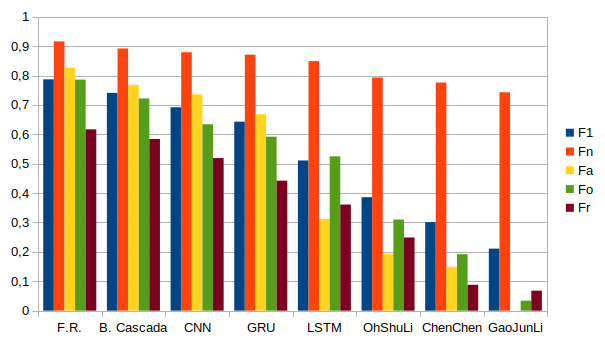
\includegraphics[scale=0.5]{img/grafica comparativa.png}
        \caption{Gráfica donde se puede apreciar de manera visual los resultados de la tabla \ref{table:Comparativa Global}}
        \label{fig:comparativa}
    \end{figure}

    

\section{Análisis}
    

    Entre los dos modelos ganadores de la competición que tenemos que según la tabla \ref{table:resultados_modelosganadores}, el que mejores resultados presenta es el clasificador basado en Random Forest. Comparando las matrices de confusión tenemos que la matriz del clasificador binario en cascada presenta más fallos al clasificar las clases \textit{FA}, \textit{Otro} y \textit{Ruido}. Esto lo podemos deducir gracias a la diagonal principal de la matriz. Por otro lado, el clasificador binario en cascada presenta una mayor tasa de aciertos en predecir los ritmos normales, sin embargo, el principal objetivo no es ese y además, el clasificador basado en Random Forest, aunque presente una menor cantidad de aciertos en clasificar ritmos normales que el otro, ocurre que el número de aciertos tampoco es que sea bajo, siendo la diferencia entre unos y otros bastante ajustada. De la matrices de confusión podemos observar un problema que atañe a ambos modelos y es la dificultad que existe a la hora de distinguir entre algunos electrocardiogramas sanos y otros que presentan un tipo de patología distinta a la fibrilación auricular. \\
    
    Los resultados de los modelos propuestos por la literatura son pésimos. Esto queda reflejado nada más ver las matrices de confusión de las tablas \ref{table:ChenChen_CM}, \ref{table:GaoJunLin_CM} y \ref{cm_ohsuli}. Observamos que el modelo GaoJunLi ha clasificado todas las instancias en una única clase, la mayoritaria. El modelo ChenChen, algo mejor que el anterior, no ha clasificado ninguna instancia como ruidosa y solo ha clasificado una instancia correcta de la clase \textit{FA}. El modelo OhShuLi solo ha sido capaz de clasificar en dos clases (Normal y ritmos con ruido ruido) dejando de lado al resto. La comparativa de los tres modelo la podemos encontrar en la tabla \ref{table:results_litera} donde vemos que el que mejores resultados presenta en términos de la métrica $F_1$ es el modelo OhShuLi. Obviamente, podemos ver que los modelos carecen de total interés. Pero indaguemos un poco más en el por qué de lo anterior.\\


    En \ref{fig:chenchen_tensorboard}, \ref{fig:gaojunli_tensorboard} y \ref{fig:ohshuli_tensorboard} presentamos del número de épocas en función del valor de la métrica. Estas curvas son bastante esclarecedoras por poner encima de la mesa el mal comportamiento de estos modelos. En la curva del modelo ChenChen, \ref{fig:chenchen_tensorboard}, observamos como la curva de entrenamiento, la naranja, crece en la primeras épocas y se mantiene oscilando pero con una tendencia constante, en cambio, la curva de validación en ningún momento aumenta. Esto nos hace ver que el modelo es incapaz de llevar a cabo un correcto aprendizaje en entrenamiento, pues los valores en el eje de ordenadas son pequeños y aún peor, que no ha sido capaz de generalizar al menos ni un poco. La gráfica del modelo OhShuLi, \ref{fig:ohshuli_tensorboard}, se ve un poco distinta a la anterior ya que la curva de validación no es constante. Podemos observar que durante las primeras épocas, el entrenamiento y la validación sí se mantuvieron constantes pero a partir de cierto momento comienzan a variar. Ambas curvas presentan una distancia muy pequeña algo que sí que es deseable, en cambio, se encuentran en un valor del eje de ordenadas insignificante, quizás más épocas hubieran sido necesarias, pero de ser así, el riesgo de sobreentrenamiento sería casi inminente. Finalmente, en la gráfica del modelo GaoJunLi, \ref{fig:gaojunli_tensorboard}, podemos apreciar una curva de aprendizaje algo más normal que las que vimos anteriormente. En las últimas épocas, la curva de entrenamiento crece abruptamente mientras la curva de validación mantiene su tendencia, lo que se puede interpretar como un posible sobreajuste. \\
    
    En resumen, los modelos propuestos por la literatura presentan malos resultados. Tenemos en cuenta que estos modelos fueron diseñados y refinados para datos pertenecientes a otra base de datos, y pese a que la finalidad haya sido la misma que la nuestra, no quiere decir que tengan que funcionar igual de bien con nuestros datos. Por otra parte comentar que el modelo ChenChen presenta bastante complejidad, es decir, demasiados grados de libertad por tener más capas convolucionales y más profundas además de dos capas LSTM con una gran cantidad de unidades. En cambio, modelo GaoJunLi puede parecer algo más simple, pues no presenta una fase de extracción de características usando CNN sino que directamente se aplican $64$ capas LSTM seguidas de capas densas, quizás este vacío haya ocasionado que únicamente clasifique según la clase mayoritaria. Aunque parezca que sea más simple, esto no quiera decir que actúe mejor, pues se piensan que $64$ capas LSTM es un número excesivo. Por otra parte, el modelo OhShuLih aunque presenta pocas capas convolucionales y de poca profundidad, el tamaño del kernel es bastante elevado. Esto hace que la extracción de características no sea fructífera, pues el tamaño de las series temporales no es demasiado grane. A todo esto se le suma la complejidad que presenta la base de datos, la cual no cuenta con una cantidad suficiente de datos y para más inri, tenemos un increíblemente fuerte desbalanceo entre clases. Todo lo anterior contribuye a que estos modelos proporcionen unos resultados bastante pobres. Esto nos sirve como ejemplo del teorema de No Free Lunch, ya que estas propuestas obtenidas de la literatura han dado buenos resultados para los problemas en los que fueron creados, pero malos resultados al realizar una tarea distinta. \\
    
    Ahora vamos a estudiar la propuestas de modelos propios. Empezamos por la selección de una hipótesis ganadora en cada modelo, para ello se han sometido cada uno a un proceso experimental en el que se ejecutan varias veces con distintos hiperparámetros. En la tabla \ref{table:model1_result} podemos observar todas las ejecuciones realizadas sobre el modelo CNN, obsevamos que el mejor valor de drop out entre los probados es de $0.4$, el número de filtros es de 235, el tamaño del kernel óptimo es de 9. En la tabla \ref{table:model2_result} podemos ver que los parámetros óptimos para el modelo LSTM son de 16 unidades en la capa de LSTM y 32 neuronas para las capas densas. Finalmente, en la tabla \ref{table:model3_result} vemos las distinta ejecuciones realizadas para el modelo GRU cuya mejor realización presenta un número de unidades GRU igual a 25 y 32 neuronas en las capas densas. \\
    
    En la tablas \ref{table:CM cnn}, \ref{table:CM lstm} y \ref{table:CM gru} presentamos las matrices de confusión de los modelos CNN, LSTM y GRU respectivamente. Observamos que ningún modelo ha sido capaz de predecir aquellos ritmos que presentan ruido y la mayoría han sido clasificados como ritmos sanos, lo cual es un desacierto pues lo que nos interesa no es saber los pacientes sanos, sino detectar los enfermos. También ocurre que todos los modelos presentan dificultad a la hora de clasificar instancias con fibrilación auricular, es decir, ninguno cumple con los objetivos que se pretendían alcanzar. Con esto vemos una clara limitación que los convierte también en modelos no deseables. \\
    
    
    En las imágenes \ref{fig:curva_model1}, \ref{fig:curva_model2} y \ref{fig:curva_model3} podemos observar las curvas de aprendizaje en las que el eje abscisas representa el número de épocas y el eje de ordenadas el valor de la métrica. En el modelo CNN podemos ver que durante las cien primeras épocas, tanto la curva de entrenamiento como la de validación van a la par. A partir de de ahí se distancian poco a poco. Mientras que la de entrenamiento adquiere una tendencia creciente, la de validación se mantiene constante. Con esto observamos que los resultados en validación no mejoran con el paso de las épocas pudiendo incurrir en sobreaprendizaje si se hubieran aplicado más épocas en el entrenamiento. La curva del modelo LSTM tiene un comportamiento muy llamativo durante las primeras épocas. Parece que no se produce un correcto entrenamiento durante las etapas más tempranas. En cambio, pasadas las primeras cien épocas, se observa que ambas curvan adquieren una tendencia creciente. Se puede también apreciar que pese a que ambas curvas sean crecientes, el incremente de la curva de entrenamiento es mayor que el de la curva de validación. Se puede llegar a pensar que más épocas hubieran hecho falta para estabilizar las curvas. Por último, las curvas del modelo GRU presentan una tendencia creciente y muy a la par. Ambas curvas no se separan demasiado la una de la otra, incluso en algunas partes podemos apreciar que la curva de validación supera a la de entrenamiento, suceso el cual no es muy normal que ocurra. \\
    
    
    En la tabla \ref{table:resultados_modelosganadores} podemos apreciar los resultados de los tres modelos que hemos propuesto. Observamos que el que mejor puntuación obtiene en todas las métricas es el modelo CNN, seguido del modelo GRU y por último, el modelo LSTM. Es interesante observar que pese a que el modelo LSTM y GRU tengan además de capas convolucionales, otras estructuras que en la teoría contribuyen al tratamiento de señales no hayan obtenido mejores resultados que el modelo puramente convolucional. Sin embargo, está bien comentar que el modelo CNN ha sido muy refinado en el proceso de experimentación por ser el más rápido en ser ejecutado, permitiendo así realizar un gran número de pruebas con diferentes hiperparámetros en pos de encontrar los óptimos. Esto mismo no ha sido posible con los otros dos modelos restantes debido a sus lentos tiempo de ejecución. Podemos llegar a pensar que tanto el modelo LSTM y GRU se hubieran podido pulir aún más para que presenten mejores resultados e incluso hubiesen podido superar al modelo CNN. \\ 
    
    
    Fijándonos en la tabla \ref{table:Comparativa Global} y a modo de conclusión, los modelos ganadores de la competición son los que mejores resultados presentan, pues fueron diseñados única y exclusivamente para esta base de datos por un equipo de profesionales cuyo objetivo era ganar la competición. El modelo RF es el mejor en todas las métricas así como el clasificador binario en cascada que es el segundo mejor en todas ellas. Los modelos empleados en la literatura, no son universales, es decir, no actúan igual de bien en todos los problemas y como consecuencia, tenemos lo sucedido. Los modelos propuestos en este trabajo no son tan sofisticados como los modelos ganadores, obteniendo peores resultados que estos, pero han sido más refinados para el problema que los encontrados en la literatura, logrando así resultados no tan malos. En la imagen \ref{fig:comparativa} podemos ver de manera visual lo anterior, aquí se aprecia todos los modelos junto con las métricas $F_1$ usadas. \\
    
    
    
\endinput